\documentclass{article}
\usepackage{style-notes}

\newcounter{lecnum} 	% define counter for lecture number
\renewcommand{\thepage}{\thelecnum-\arabic{page}}	% define how page number is displayed (< lecture number > - < page number >)
% define lecture header and page numbers
% NOTE: to call use \lecture{< Lecture # >, < Lecture name >, < Chapter # >, < Chapter name >, < Section #s >}
\newcommand{\lecture}[5]{

    % define headers for first page
    \thispagestyle{empty} % removes page number from page where call is made

    \setcounter{lecnum}{#1}		% set lecture counter to argument specified

    % define header box
    \begin{center}
    \framebox{
      \vbox{\vspace{2mm}
    \hbox to 6.28in {\textbf{MATH 320: Probability} \hfill}
       \vspace{4mm}
       \hbox to 6.28in {{\hfill \Large{Lecture #1: #2} \hfill}}
       \vspace{2mm}
       \hbox to 6.28in {\hfill Chapter #3: #4 \small{(#5)}}
      \vspace{2mm}}
    }
    \end{center}
    \vspace{4mm}
    
    % define headers for subsequent pages
    \fancyhead[LE]{\textit{#2} \hfill \thepage} 		% set left header for even pages
    \fancyhead[RO]{\hfill \thepage}		% set right header for odd pages

}


% define macros (/shortcuts)
\newcommand{\bu}[1]{\textbf{\ul{#1}}}			% shortcut bold and underline text in one command
\newcommand{\blankul}[1]{\rule[-1.5mm]{#1}{0.15mm}}	% shortcut for blank underline, where the only option needed to specify is length (# and units (cm or mm, etc.)))
\newcommand{\vecn}[2]{#1_1, \ldots, #1_{#2}}		% define vector (without parentheses, so when writing out in like a definition) of the form X_1, ..., X_n, where X and n are variable. NOTE: to call use $\vecn{X}{n}$
\newcommand{\comp}{{\sim}}						% shortcut for tilde without extra space, using for complement


% NOTES on what didn't cover



\begin{document}

\lecture{4}{Conditional Probability}{1}{Probability}{1.3}

In some probability problems a condition is given which restricts your attention to a subset of the sample space.\bigskip

\bu{Conditional probability by counting}\bigskip

Motivating example\bigskip
\begin{itemize}
    \item Example: Roll a die. $A = \{1, 2, 3, 4\}$ and $B = \{4, 5, 6\}$.
    \item[] We have the following probabilities: \hspace{10pt}$P(A) = $ \hspace{50pt} $P(B) = $\\
    \item[] If we know that $A$ already occurred, what is the probability of $B$?\\
    \item This is known as a \blankul{3cm} probability.
\end{itemize}\vspace{90pt}

Updated sample spaces\bigskip
\begin{itemize}
    \item The \blankul{3cm} is the set of all possible outcomes.
    \item[] In other words, only the outcomes in the sample space can be \blankul{2cm}.\\
    \item When an \blankul{4cm}, we don't know specifically which outcome was observed.\\
    \item `$A$ occurred' means we know that the outcome is one of the elements in \blankul{1cm}. That is, there is no chance to get outcomes \blankul{2cm}.
    \item[] So these numbers are \blankul{2cm} from the sample space.\\
    \item Thus, an event which already occurred \blankul{2cm} the sample space and it becomes an \blankul{2cm} sample space.
\end{itemize}\bigskip

Examples with contingency tables\bigskip
\begin{itemize}
    \item Example: Here is attendance and college major of students:
    \begin{center}
        \begin{tabular}{| c | c | c | c || c |}
        \hline
         & Statistics & Art & Chemistry & Total\\
        \hline
        Perfect & 100 & 40 & 80 & 220\\
        \hline
        Good & 20 & 50 & 70 & 140\\
        \hline
        Poor & 30 & 15 & 30 & 75\\
        \hline\hline
        Total & 150 & 105 & 180 & 435\\
        \hline
        \end{tabular}%https://tex.stackexchange.com/questions/130818/how-to-draw-a-double-hline-in-a-table-without-interrupting-vertical-lines
    \end{center}\bigskip
    \item Suppose we are told the selected student has good attendance, what is the probability the student is a chemistry major?\\
    \item[] Said equivalently: What is the probability the student is a chemistry major \textit{given that the student has good attendance}?\vspace{100pt}
    \item[] Another way we could interpret this result is: Of students with Good attendance, \blankul{1.5cm} are Chemistry majors.\\
    \item Thus the restricted sample space still applies to contingency tables, where now we look only within a single row or column because we have additional (GIVEN) information.
    \item[] And we see that these conditional probability problems could also be solved using probabilities.\bigskip
    \item Types of probabilities:
    \begin{itemize}
        \item \textbf{Marginal probabilities}: Refer to one event; use column / row totals to find these.
        \item \textbf{Joint probabilities}: Refer to two (or more) events; use numbers in the middle of the table to find these.
        \begin{figure}[H]
            \center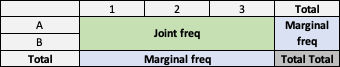
\includegraphics[scale=0.7]{test-1/general-contingency-table}
        \end{figure}
        \item Examples: $P(\text{Stats}) = $\hspace{100pt} $P(\text{Perfect} \cap\text{Stats}) = $
    \end{itemize}
\end{itemize}\bigskip

\newpage

\bu{Defining conditional probability}\bigskip

\begin{itemize}
    \item The previous examples showed two natural ways of finding conditional probability. The first was based on counting and the second on probabilities.\\
    \item \textbf{Conditional probability by counting for equally likely outcomes}\bigskip
    \item[] $P(A \mid B) = $\bigskip
    \item[] When outcomes are not equally likely, this rule does not apply. Then we need a general definition of conditional probability.\\
    \item Definition: The \textbf{conditional probability} of an event $A$ given the occurrence of the event $B$ is:\\
    \item[] $P(A \mid B) = $\\
    \item The notation $P(A \mid B)$ is read ``the conditional probability of $A$ given $B$''.
    \begin{itemize}
        \item $A$ is the main event of interest and $B$ is called the conditioning event.
    \end{itemize}
\end{itemize}\bigskip

Examples\bigskip
\begin{enumerate}
    \item 100 cars will be painted in a production line. Of these cars 25 will be painted blue, 75 will be painted red, 12 will get a clear coat, and 9 of the blue cars will get a clear coat at random.\vspace{70pt}
    \begin{enumerate}
        \item What is the probability that a car will be painted blue?\vspace{30pt}
        \item Given that a car is blue, what is the probability that it got a clear coat?\vspace{30pt}
        \item What is the probability that the car is red, given that it did not get a clear coat?\vspace{30pt}
    \end{enumerate}
    \item A pair of fair four sided dice is rolled and the sum is determined. Find the probability that a sum of 3 is rolled given that a sum of 3 or 5 is rolled.\vspace{120pt}
    \item Probabilities for the number of auto insurance claims are given in the table below.\\
    \begin{center}
        \begin{tabular}{| l || c | c | c | c |}
        \hline
        Number of claims & 0 & 1 & 2 & 3\\
        \hline
        Probability & 0.72 & 0.22 & 0.05 & 0.01\\
        \hline
        \end{tabular}
    \end{center}\bigskip
    \item[] Find the probability that a policyholder files exactly 2 claims, \textit{given that the policy holder has filed at least one claim}.\vspace{120pt}
    \item[] This tells us $\approx$ \blankul{1cm} of policyholders who file a claim file exactly 2 claims.
\end{enumerate}\bigskip

\begin{itemize}
    \item Note on conditional probability:\\
    \begin{itemize}
        \item ALWAYS $P(B \mid A) = $\\
        \item ONLY SOMETIMES $P(B \mid A) = $\\
    \end{itemize}
\end{itemize}

\newpage

\bu{Applying conditional probability}\bigskip

Probability rules for conditional probability\bigskip
\begin{itemize}
    \item All of the rules (axioms) for a probability assignment from ``Lecture 3 -- Probability'' apply to a conditional probability function $P(\,\cdot \mid B)$ as well.
    \item In addition, the theorems we proved also hold true for $P(\,\cdot \mid B)$.\bigskip
    \item Examples and (a few) new theorems:\bigskip
    	\begin{itemize}
             \item We know $P(\comp A) = 1 - P(A)$, using the previous example we can find $P(\comp 2 \mid C)$.\vspace{50pt}
             \item[] In general: $P(\comp{A} \mid B) = $\\
             \item We know $P(A \cup B) = P(A) + P(B) - P(A \cap B)$. Now applying this to the conditional probability of $A \cup B$ given $C$,\bigskip
             \item[] $P(A \cup B \mid C) = $\bigskip
         \end{itemize}
\end{itemize}\bigskip

Multiplication rule for probability\bigskip
\begin{itemize}
    \item The definition of conditional probability can be rewritten as a multiplication rule for probabilities, where we are trying to get an expression for the joint probability of $A$ and $B$.\vspace{40pt}
    \item \textbf{Multiplication rule for probability}: Given events $A$ and $B$,\bigskip
    \item[] $P(A \cap B) = $\\
    \item[] $P(A \cap B) = $\\
    \item Interpretation:\vspace{50pt}
    \item Example: At a country fair game there are 25 balloons on a board of which 10 balloons are yellow, 8 are red and 7 are green. A player throws darts at balloons to win a prize and randomly hits one of them. If a player throws two darts in a row what is the probability that both balloons hit are yellow?\vspace{140pt}
    \item[] The ``direct way'' of solving counting probability problems is just an application of the multiplication rule for probability.
    \item Often in a probability experiment, it can be easier to assign $P(A)$ and $P(B \mid A)$ rather than $P(A \cap B)$. Then we can easily compute $P(A \cap B)$ using these.
    \item[] Example: Two cards are drawn at random from a standard deck without replacement, as in the previous example. Find the probability that both are kings.\vspace{30pt}
    \item This multiplication rule can be extended to any number of events as well.
    \begin{itemize}
        \item More generally, given $k$ events $\vecn{A}{k}$\bigskip
        \item[] $P(A_1 \cap \dots \cap A_k) = $\bigskip
        \item Example: For $k = 3$ events, the multiplication rule is\bigskip
        \item[] $P(A_1 \cap A_2 \cap A_3) = $
    \end{itemize}\bigskip
    \item Example:
        \begin{enumerate}[(a)]
            \item From an ordinary deck of playing cards, cards are to be drawn successively at random and without replacement. What is the probability that the third spade appears on the sixth draw?\vspace{45pt}
            \item Same question as (a), except now with replacement.\vspace{20pt}
    \end{enumerate}
\end{itemize}\bigskip

Using tree diagrams in probability problems\bigskip
\begin{itemize}
    \item Experiments involving multiple stages, such as drawing two cards without replacement can be summarized completely using trees!
    \item Examples:
    \begin{enumerate}
        \item Lets continue the drawing two kings example from before:\vspace{150pt}
        \begin{enumerate}
            \item What is the probability of exactly one king?\vspace{120pt}
            \item What is the probability of two kings or no kings?\vspace{50pt}
            \item What is the probability of at least one king?\vspace{60pt}
            \item[] Can easily use \blankul{3cm} rather than solving for many branches.\\
            \item Find the probability that the second card is a king $(K2)$, given that the first card drawn was a king.\vspace{30pt}
        \end{enumerate}
     \end{enumerate}
     \begin{itemize}
        \item This is just knowing parts of the tree. For problems that are just asking for ``one level'' of the tree or ``one stage'' of an experiment, it is often easier to find conditional probability by
        \item[] (1) Taking into account the information by updating the scenario and then \\(2) Solving like normal.
    \end{itemize}\bigskip
    \item Creating tree diagram and summing up the final probabilities of interest simplifies many harder problems!
    \item[] In most experiments, there will be a natural order of events, which will make setting up the tree intuitive.
    \item General tree
    \begin{figure}[H]
        \center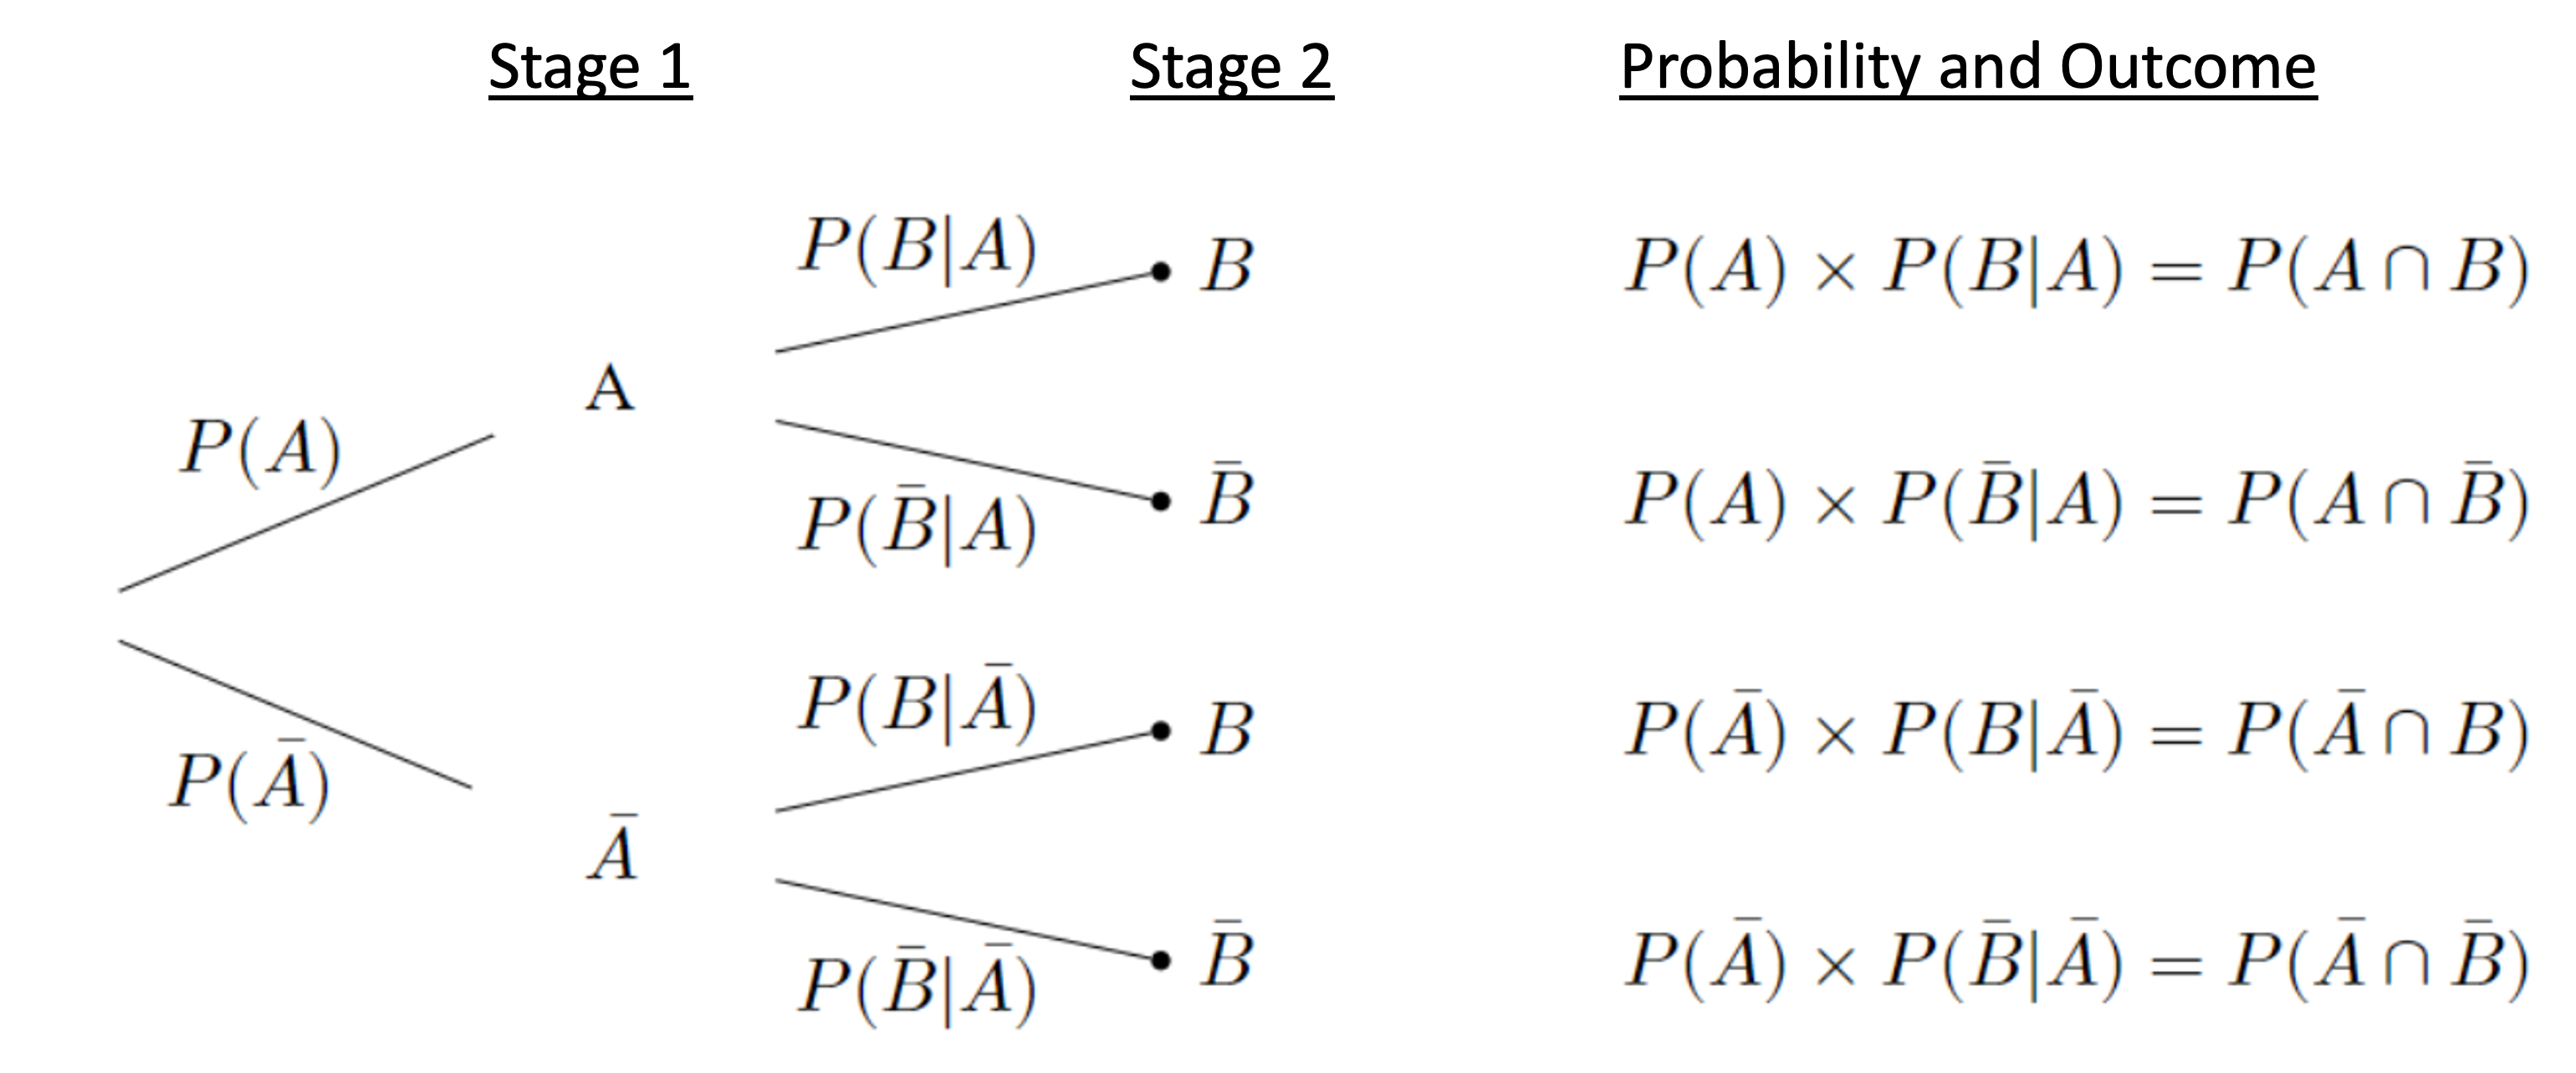
\includegraphics[scale=0.5]{test-1/general-tree}
    \end{figure}\bigskip
    \begin{enumerate}\setcounter{enumi}{1}
        \item There are two jars, Jar 1 and Jar 2. Jar 1 has 6 red and 5 white chips and Jar 2 has 8 red and 7 white chips.
        \begin{enumerate}
            \item If you first pick a red chip from Jar 1 and transfer the chip to Jar 2, what is the probability of then picking a red chip from Jar 2?\vspace{50pt}
            \item If you first pick a chip (don't know which color) from Jar 1 and transfer the chip to Jar 2, what is the probability of then picking a red chip from Jar 2?\vspace{100pt}
        \end{enumerate}\newpage
        \item An insurance company sells several types types of insurance policies including auto policies and homeowner policies.
        \begin{itemize}
            \item Let $A$ be those people with an auto policy only and $P(A) = 0.3$
            \item Let $H$ be those people with an homeowner policy only and $P(H) = 0.2$
            \item Let $A$+$H$ be those people with both an auto and homeowner's policy (but no other policies) and $P(A\text{+}H) = 0.2$
        \end{itemize}
        \item[] Further let $R$ be the event that the person will renew at least one of these policies. From past experience the following conditional probabilities are assigned: \medskip\\$P(R \mid A) = 0.6, P(R \mid H) = 0.7$ and $P(R \mid A \text{+} H) = 0.8$.
        \item[] Given that a person selected at random has an auto or homeowner policy, what is the conditional probability that a person will renew at least one of those policies?
    \end{enumerate}
\end{itemize}\bigskip

\end{document}